\section{Parallel with Discrete Fourier Transform}
\label{app:fourier_t}

Pour développer l'intuition, et voir plus clairement le parallèle avec la transformée de Fourier discrète, il peut être intéressant de se demander si un graphe permet de retrouver l'interprétation habituelle de la transformée de Fourier discrète d'un signal temporel. Les graphes cycliques permettent cela. En effet, soit un signal $x$ sur le graphe cycle à $N$ sommets $C_N$. La matrice laplacienne $L_N$ de ce graphe s'écrit, pour $N=6$ 
\[ L_6 := 
\begin{bmatrix}
2 & -1 & 0 & 0 & 0 & -1 \\
-1 & 2 & -1 & 0 & 0 & 0 \\
0 & -1 & 2 & -1 & 0 & 0 \\
0 & 0 & -1 & 2 & -1 & 0 \\
0 & 0 & 0 & -1 & 2 & -1 \\
-1 & 0 & 0 & 0 & -1 & 2 \\
\end{bmatrix}
\]
En notant
\[J_N :=
\begin{bmatrix}
0 & 1 & 0 & \dots & 0 \\
0 & 0 & 1 & \dots & 0 \\
\vdots  &     &     & \ddots & \vdots  \\
0 & & &        & 1 \\
1 & 0 & 0 & \dots  & 0
\end{bmatrix}
\]
on observe que 
\begin{align}
    L_N = 2I_N - J_N - J_N^{N-1}
\end{align}
Or les valeurs propres de $J$ sont les racines $N$-ièmes de l'unité $\omega^0,...,\omega^{N-1}$ où $\omega := e^{\frac{2i\pi}{N}}$ et pour tout $k\in [\![0,N-1]\!]$, \[X_k := \begin{bmatrix} 1 \\\omega^k \\ \omega^{2k}\\ \vdots\\ \omega^{(N-1)k}\end{bmatrix}\]
est vecteur propre de $J$ associé à la valeur propre $\omega^k$.
Cela permet donc, en notant $W$ la matrice de transformée de Fourier discète
\[ W :=
\begin{bmatrix}
1&1&1&1&\cdots &1 \\
1&\omega&\omega^2&\omega^3&\cdots&\omega^{N-1} \\
1&\omega^2&\omega^4&\omega^6&\cdots&\omega^{2(N-1)}\\ 1&\omega^3&\omega^6&\omega^9&\cdots&\omega^{3(N-1)}\\
\vdots&\vdots&\vdots&\vdots&\ddots&\vdots\\
1&\omega^{N-1}&\omega^{2(N-1)}&\omega^{3(N-1)}&\cdots&\omega^{(N-1)(N-1)}
\end{bmatrix}
\]
d'écrire
\begin{align}
    L_N = W(2I_N -\Omega-\Omega^{N-1})W^{-1}
\end{align}
où $\Omega := Diag(w^0,...,w^{N-1})$\\
Ainsi, les valeurs propres de $L_N$ sont les $\lambda_k = 2 - \omega^k - \omega^{-k}$ pour $k \in [\![0,N-1]\!]$.\\
En utilisant la définition de la transformée de Fourier sur les graphes \ref{eq:GFT}, on explicite le $k$-ième coefficient de Fourier
\begin{align}
    \Tilde{x}_k &= W_k^*x\\
    &= \overline{W_k}x\\
    &= \sum_{n=0}^{N-1}x_n\omega^{-nk} \\
    &= \sum_{n=0}^{N-1}x_n e^{-2i\pi n\frac{k}{N}}
\end{align}
On retrouve la définition de la transformée de Fourier discrète.

\begin{figure}[h]
  \centering
  \begin{subfigure}{0.35\linewidth}
    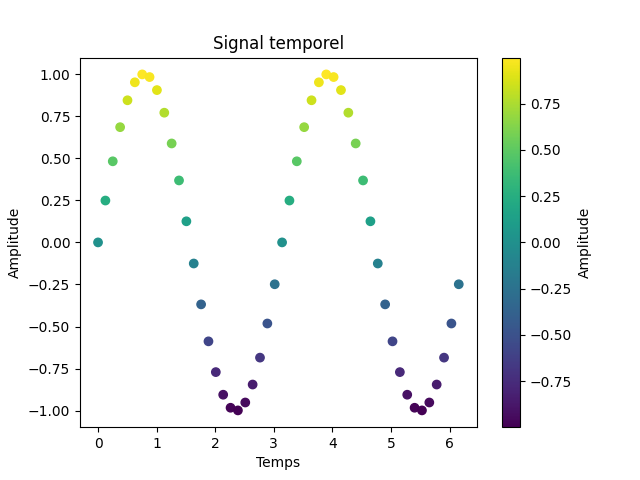
\includegraphics[width=6.5cm]{img/temporal_signal.png}
    \caption{Représentation temporelle d'un signal echantillonné}
    \label{fig:DANN_1}
  \end{subfigure}
  \hspace{1.5cm}
  \begin{subfigure}{0.35\linewidth}
    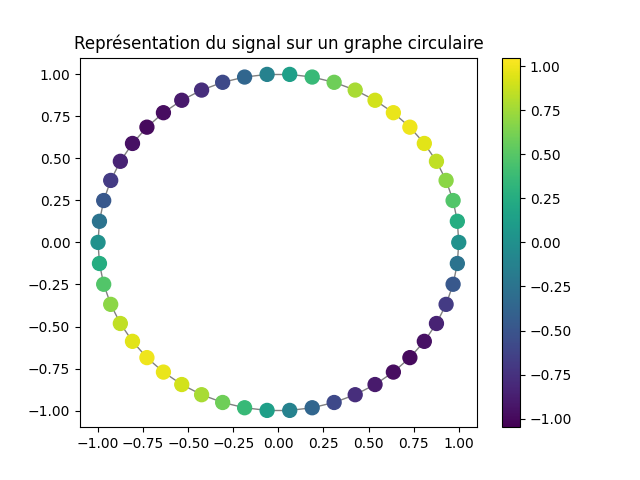
\includegraphics[width=6.5cm]{img/graph_signal.png}
    \caption{Représentation du même signal sur un graphe circulaire}
    \label{fig:DANN_2}
  \end{subfigure}
  \caption{Deux représentations d'un signal échantillonné dont on calcule la transformée de Fourier par les deux définitions dont on dispose : la transformée de Fourier discrète, et la transformée de Fourier d'un graphe}
  \label{fig:DANN
}
\end{figure}